\begin{figure}[t]
    \centering
    \resizebox{\textwidth}{!}{
    \begin{tikzpicture}

    \node (ligne_1) at (0, 0) {};

    \node[] at ($(ligne_1) + (-4.5cm, 0cm)$) {
    \begin{minipage}{4.5cm}
        \centering
        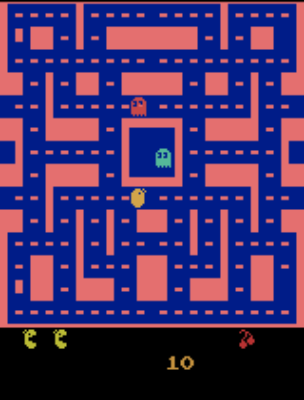
\includegraphics[width=2cm]{figures/clustering_agent_representation/pictures/ms_pacman/qualitative/cluster_1/image_1.png}
        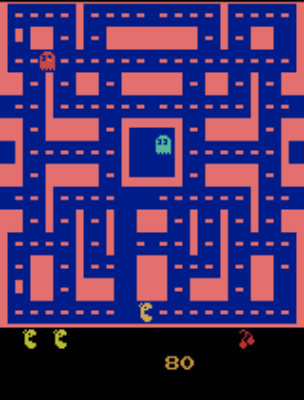
\includegraphics[width=2cm]{figures/clustering_agent_representation/pictures/ms_pacman/qualitative/cluster_1/image_2.png}

        \small Start of the episode.
    \end{minipage}
    };

    \node[] at ($(ligne_1) + (0cm, 0cm)$) {
    \begin{minipage}{4.5cm}
        \centering
        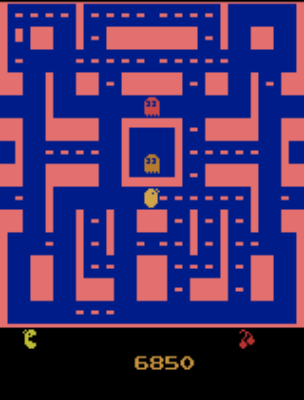
\includegraphics[width=2cm]{figures/clustering_agent_representation/pictures/ms_pacman/qualitative/cluster_0/image_1.png}
        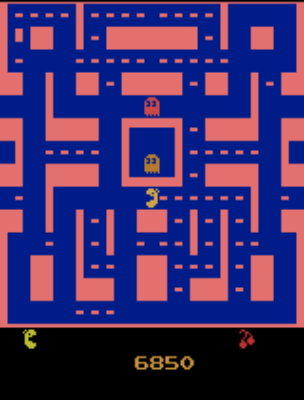
\includegraphics[width=2cm]{figures/clustering_agent_representation/pictures/ms_pacman/qualitative/cluster_0/image_2.png}

        \small Middle of the episode.
    \end{minipage}
    };

    \node[] at ($(ligne_1) + (4.5cm, 0cm)$) {
    \begin{minipage}{4.5cm}
        \centering
        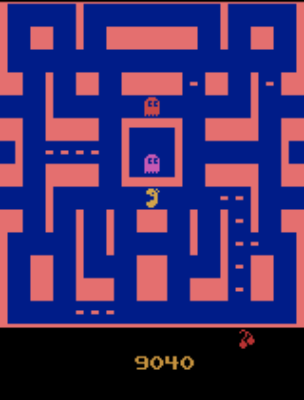
\includegraphics[width=2cm]{figures/clustering_agent_representation/pictures/ms_pacman/qualitative/cluster_2/image_1.png}
        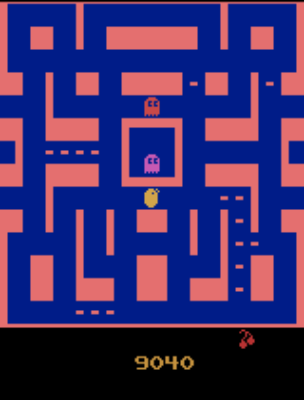
\includegraphics[width=2cm]{figures/clustering_agent_representation/pictures/ms_pacman/qualitative/cluster_2/image_2.png}

        \small End of the episode.
    \end{minipage}
    };

    \end{tikzpicture}
    }
    \caption{Clusters identified by \gls{car} in the Ms.\ Pac-Man environment (layer 6b, $K=3$).}
    \label{fig:qualitative_ms_pacman}
\end{figure}
